\documentclass[a4paper,12pt]{report}


\usepackage[english,romanian]{babel}
\usepackage{pgfpages}
\usepackage{graphicx}

\usepackage{ucs}
\usepackage[utf8x]{inputenc}

\newcommand{\texten}[1]{\foreignlanguage{english}{#1}}
\newcommand{\textro}[1]{\foreignlanguage{romanian}{#1}}

\newcommand{\sh}[0]{\textcommabelow{s}}		%pentru ş cu virgulă
\newcommand{\tz}[0]{\textcommabelow{t}}		% pentru ţ cu virgulă

\usepackage[unicode]{hyperref}
\usepackage[T1]{fontenc}
\usepackage{tikz}
% \usepackage{colortbl}
%\usepackage{yfonts}

\usepackage{amssymb,amsmath}
\usepackage{amsthm}

% \usepackage{paralist}

\usepackage{enumerate}

\usepackage{makeidx}
\usepackage{showidx}

% \usepackage{float}

% \usepackage{subfig}

% \usepackage{multirow}
% \usepackage{rotating}

% \usepackage[ruled,vlined,longend]{algorithm2e}
% \SetAlFnt{\small}

\usepackage{program}

\usepackage{verbatim}

\usepackage{listings}

\lstset{
	language=C,
%	basicstyle=\ttfamily,
	basicstyle=\small\ttfamily,
	keywordstyle=\bfseries,
	commentstyle=\itshape,
	escapechar=\,
	emphstyle=\bfseries\color{red}
 	commentstyle=\slshape\color{green!50!black},
 	keywordstyle=\bfseries\color{blue!50!black},
 	identifierstyle=\color{blue},
 	stringstyle=\color{orange},
}

\usepackage{setspace}
% \usepackage{tocbibind}
% \usepackage{fancyhdr}

\usepackage{hyperref}


% \newcommand{\OSName}{\textit{Nachos}}
\newcommand{\OSName}{\textit{OrionOS}}

\title{The Design of \OSName{} Operating System}

\author{Pană, A., Soucup A., Vultur H., Zene, A. }

\onehalfspacing

\begin{document}

\selectlanguage{english}
% \selectlanguage{romanian}


\maketitle

\begin{abstract}
	A short description of this report content. 
	
	Take into account that a design document is a complete high-level solution to the problem presented. It should be detailed enough that somebody who already understands the problem could go out and code the project without having to make any significant decisions. Further, if this somebody happens to be an experienced coder, they should be able to use the design document to code the solution in a few hours (not necessarily including debugging). 
\end{abstract}


\chapter{General Presentation}

\section{Working Team}

\begin{enumerate}
	\item Pană Alexandru
	    \begin{enumerate}
	     \item Threads: dealt with synchronisation mechanisms implementation \& priority donation
	     \item Userprog: dealt with file system syscalls
	     \item Virtual Memory: dealt with swapping
	    \end{enumerate}

	\item Soucup Adrian
	    \begin{enumerate}
	     \item Threads: dealt with advanced scheduler
	     \item Userprog: dealt with wait syscall
	     \item Virtual Memory: Memory Mapped files
	    \end{enumerate}
	    
	\item Vultur Horațiu
	    \begin{enumerate}
	     \item Threads: dealt with priority scheduler
	     \item Userprog: dealt with argument passing, process termination messages \& exec syscall
	     \item Virtual Memory: Stack growth
	    \end{enumerate}

	\item Zene Andrei
	    \begin{enumerate}
	     \item Threads: dealt with alarm clock \& fixed-point arithmetic
	     \item Userprog: dealt with exit syscall, process data structures \& denying writes to executables
	     \item Virtual Memory: Paging (lazy-loading \& Frame table management)
	    \end{enumerate}
	   
\end{enumerate}


% \section{System}



\chapter{Design of Module \textit{threads}}

\section{Alarm clock}

    \subsection{Initial Functionality}

	At the beginning of this project the function \textit{sleep\_timer} is implemented as a busy wait. We want to reimplement it to avoid the busy wait.

    \subsection{Data Structures and Functions}

    \begin{lstlisting}
	struct thread
	{

	      ...
	  /* the time (in number of ticks) at which a 
	      sleeping thread should wake up */
	      int64_t wakeup_time;		
	      ...

	};
	
	/* a sorted list containing all sleeping 
	(blocked) threads. Sorting is done using 
	thread_wakeup_time_comparison function*/
	static struct list sleep_list;

	/* comparison function to order the sleeping
	threads ascending by their wakeup time */
	list_less_func thread_wakeup_time_comparison;

	/* sets the time at which the thread should 
	wake up and puts the thread in the sleeping 
	threads list */
	void thread_sleep (int64_t wakeup_time);

	/*this function checks if there are sleeping
	threads that should wake up at this moment 
	and calls the function thread_unblock for 
	each of those threads.*/
	void handle_sleeping_threads();    
    \end{lstlisting}


    \subsection{Functionality}

	When the function \textit{sleep\_timer} is called, this function calculates the time (in ticks) at which the thread should wake up, sets this time in the thread structure, inserts the thread in a sleeping list and then calls \textit{thread\_block}, in order to set the status THREAD\_BLOCKED, and to call the scheduler. The sleeping list is sorted ascending according to the time at which the threads should wake up (the first thread in this list is the thread that should wake up the earliest). At every timer interrupt, the function \textit{handle\_sleeping\_threads} is called which checks if there are threads that can wake up at the current moment of time. If there are, these threads are removed from the sleeping list, and \textit{thread\_unblock} is called on them, which sets their status to THREAD\_READY and puts them in the ready list.

	In order to avoid race conditions, the interrupts are disabled during the execution of \textit{sleep\_timer} and \textit{timer\_interrupt}.

    %\begin{figure}[h]
    %	\centering
    %	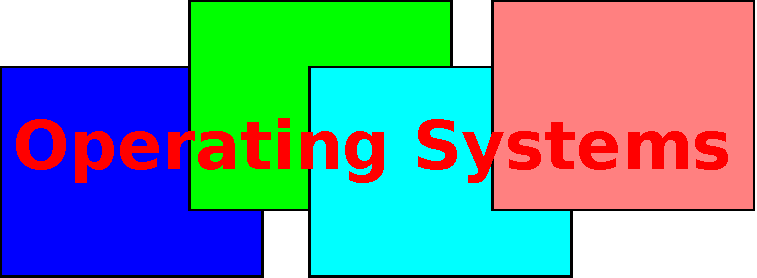
\includegraphics[width=0.5\textwidth]{figures/sample-image.pdf}
    %	\caption{Sample image}
    %	\label{fig:sample-image}
    %\end{figure}


    %Here you have a pseudo-code description of an algorithm taken fom \\ \href{http://en.wikibooks.org/wiki/LaTeX/Algorithms\_and\_Pseudocode\#Typesetting\_using\_the\_program\_package}{http://en.wikibooks.org/wiki/LaTeX}. It uses the \textit{program} package. Alternatively, you can use \textit{algorithmic} or \textit{algorithm2e} packages. 

    %\begin{program}
    %\mbox{Example of a pseudo-code algorithm description:}
    %\BEGIN %
    %  \FOR i:=1 \TO 10 \STEP 1 \DO
    %     |expt|(2,i); \\ |newline|() \OD %
    %\rcomment{This text will be set flush to the right margin}
    %\WHERE
    %\PROC |expt|(x,n) \BODY
    %          z:=1;
    %          \DO \IF n=0 \THEN \EXIT \FI;
    %             \DO \IF |odd|(n) \THEN \EXIT \FI;
    %\COMMENT{This is a comment statement};
    %                n:=n/2; x:=x*x \OD;
    %             \{ n>0 \};
    %             n:=n-1; z:=z*x \OD;
    %          |print|(z) \ENDPROC
    %\END
    %\end{program}


    \subsection{Design Decisions}

	This solution has the advantage that the time spent in the \textit{timer\_interrupt} function is constant, because the list is ordered. On the other hand the time spent for inserting is O(n), because we use a list to keep the threads. A better solution would be to use a heap as a data structure to keep the sleeping threads. In this way, the insertion timewould be only O(log n). 

	However, this solution is better than the solution in which at every \textit{timer\_interrupt} the whole sleeping list is traversed to see if there is a thread that should wake up even though the insertion is done in constant time, (without sorting the list) because \textit{timer\_interrupt} is called more often than the function \textit{sleep\_timer}.

    \subsection{Tests}

    alarm-single, alarm-multiple, alarm-negative, alarm-simultaneous, alarm-zero



\section{Priority scheduler}

    \subsection{Initial Functionality}

	At the beginning of this project the scheduler is implented as a Round-Robin scheduler. We want to reimplement it as a priority scheduler.

    \subsection{Data Structures and Functions}

    \begin{lstlisting}
      struct thread
      {
	    ...
	  /*the fixed priority of the thread,
	  given at creation */
	  int priority;
	  
	  /* the priority at a given moment of
	  the thread. This can be either the
	  thread's fixed priority or the 
	  priority inherited by donation */
	  int current_priority;		
	    ...
      };

      /* ready_list[i] contains the threads of
      priority i having the status THREAD_READY. */
      static struct list ready_list[PRI_MAX + 1];

      /* the priority scheduler */
      static struct thread * next_thread_to_run (void);

      /* promotes a thread to current thread's priority */
      void thread_promote (struct thread *);
      
      /* forces the current thread to return to it's
      default fixed priority. */
      void thread_lessen ();

      /* reimplementation of thread_unblock which checks 
      if the new READY thread is more prioritary than the 
      current thread, and if so, it forces current thread 
      to yield the cpu. */
      void thread_unblock (struct thread *);

      struct lock 
      {
	  struct thread *holder;   /* Thread holding lock */
	  unsigned value;          /* Current value. */
	  struct list waiters;     /* List of waiting threads. */
      };

      /* reimplementation of old lock functions according to
      the new structure of the lock */
      void lock_init (struct lock *);
      void lock_acquire (struct lock *);
      bool lock_held_by_current_thread (const struct lock *);

      /* reimplementation of old lock_acquire, with priority
      donation. When the lock is hold by a less prioritary
      thread, that thread is promoted to current thread's
      priority. */
      bool lock_try_acquire (struct lock *);

      /* reimplementation of old lock_release, with priority
      donation. If current thread was promoted, it gives up
      to it's inherited priority after releasing the lock. */
      void lock_release (struct lock *);      

    \end{lstlisting}


    \subsection{Functionality}

	The ready list is organized as a vector of lists, in which, every list contains threads that have the same priority. The scheduler calls the function \textit{next\_thread\_to\_run} which pops the most prioritary thread from its list and returns it; if there are more threads with the same priority, a round-robin algorithm is used. In order to avoid priority inversion, the \textit{lock\_aquire} is rewritten, so that whenever a thread with a greater priority waits for a lock holded by a thread with a lower priority, the function \textit{lock\_aquire} calls the function \textit{thread\_promote (holder)}. The function \textit{thread\_promote} sets the new current priority  for the holder to the priority of the current thread and then moves the thread in the ready lists vector from its list to the beginning of the list corresponding to its new priority. At the next call of the scheduler, the thread that holds the lock will receive cpu, and will be able to release the lock. In order to bring things back to previous situation, the function \textit{lock\_release} is rewritten, so that it calls the function \textit{thread\_lessen}, which forces the current thread to go back to its fixed priority, and to yield the cpu. At the call of \textit{thread\_yield} the next thread will put itself in the ready list corresponding to its previous priority. 

	To be able to give the cpu to a new more prioritary thread when it occurs, the \textit{thread\_unblock} function is rewritten to do this test, and force current thread to yield the cpu if necessary.

	In order to avoid race conditions, the interrupts are disabled during the execution of \textit{thread\_promote} and \textit{thread\_lessen}, and of course during the execution of functions where it was previously disabled.

    %\begin{figure}[h]
    %	\centering
    %	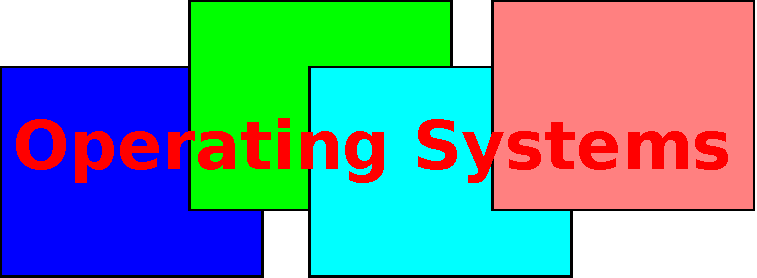
\includegraphics[width=0.5\textwidth]{figures/sample-image.pdf}
    %	\caption{Sample image}
    %	\label{fig:sample-image}
    %\end{figure}


    %Here you have a pseudo-code description of an algorithm taken fom \\ \href{http://en.wikibooks.org/wiki/LaTeX/Algorithms\_and\_Pseudocode\#Typesetting\_using\_the\_program\_package}{http://en.wikibooks.org/wiki/LaTeX}. It uses the \textit{program} package. Alternatively, you can use \textit{algorithmic} or \textit{algorithm2e} packages. 

    %\begin{program}
    %\mbox{Example of a pseudo-code algorithm description:}
    %\BEGIN %
    %  \FOR i:=1 \TO 10 \STEP 1 \DO
    %     |expt|(2,i); \\ |newline|() \OD %
    %\rcomment{This text will be set flush to the right margin}
    %\WHERE
    %\PROC |expt|(x,n) \BODY
    %          z:=1;
    %          \DO \IF n=0 \THEN \EXIT \FI;
    %             \DO \IF |odd|(n) \THEN \EXIT \FI;
    %\COMMENT{This is a comment statement};
    %                n:=n/2; x:=x*x \OD;
    %             \{ n>0 \};
    %             n:=n-1; z:=z*x \OD;
    %          |print|(z) \ENDPROC
    %\END
    %\end{program}


    \subsection{Design Decisions}

	why promoting/lessening is done in \textit{lock\_aquire} / \textit{lock\_release}?
	
	why vector of lists?

    \subsection{Tests}

	alarm-priority, priority-change, priority-condvar, priority-donate-chain, priority-donate-lower, priority-donate-multiple, priority-donate-nest, priority-donate-one, priority-donate-sema, priority-fifo, priority-preempt, priority-sema

\section{Advanced scheduler}

    \subsection{Initial Functionality}

	At the beginning of this project the scheduler is implented as a priority scheduler. We want to reimplement it as an advanced scheduler(4.4BSD).

    \subsection{Data Structures and Functions}

    \begin{lstlisting}

      struct thread
      {
	    ...
	  /* */
	  int nice;
	  /* */
	  int64_t current_cpu;  
	    ...
      };      

      /* load average of the whole system */
      int64_t load_avg;

    \end{lstlisting}


    \subsection{Functionality}

	\begin{program}
	\mbox{The timer\_interrupt function modification:}     
	\PROC |timer\_interrupt|() \BODY
		recent\_cpu[running\_thread]:=recent\_cpu[running\_thread] + 1;
		\IF TIMER\_FREQ \% TIMER\_TICKS \EQ 0 
		      \THEN thread\_for\_each(all\_threads\_list, thread\_recompute\_priority); 
		      \ELSE thread\_recompute\_priority(running\_thread);
		\FI;
	\END;
	\PROC |thread\_recompute\_priority|(thread) \BODY
		ready\_threads = count(ready\_list);
		\mbox{Use functions from fixed-point.h lib to compute the next expressions};
		load\_avg:= (59/60) * load\_avg + (1/60)*ready_threads; 
		recent\_cpu[thread]:= (2*load\_avg)/(2 * load\_avg + 1) + recent\_cpu[t] + nice[t];
		new\_priority:=clamp(PRI\_MAX - (recent\_cpu / 4) - (nice * 2));
		old\_priority:=priority[thread];
		\IF new\_priority != old\_priority
		      \THEN remove(ready\_list[old\_priority], thread.elem);
			    push\_back(ready\_list[new\_priority], thread.elem);
		\FI;
	\END;
	\end{program}

	It is important that computations for recent\_cpu and load\_avg are done with functions from fixed\_point.h, because these two variables are real numbers.

	In order to be able to choose between the MLFQS scheduler and the Priority Scheduler when running the tests, the thread\_mlfqs flag is used. If this flag is set, the functions 
	\begin{itemize}
	  \item \textit{thread\_create} ignores the priority given as a parameter, and creates a thread with priority PRI\_DEFAULT,
	  \item \textit{thread\_set\_priority}, does not change the priority anymore
	  \item \textit{lock\_aquire} and \textit{lock\_release} don't do priority donation anymore
	\end{itemize}

    \subsection{Design Decisions}


    \subsection{Tests}



\chapter{Design of Module \textit{userprog}}


\section{Initial Functionality}

Describe briefly what you have been given (have started from) at the beginning of the assignment and the way the existing functionality must be extended.

\section{Data Structures and Functions}

Specify the \textit{data structures} and \textit{functions} involved in your solution and what are they used for. Describe in few words the purpose of new added data structures, fields and functions. 

\begin{lstlisting}
	struct existent_data_structure {
		int newField;
	};
	
	struct newDataStructure {
	};
	
	int newFunction();
\end{lstlisting}


\section{Functionality}

Describe \textbf{briefly}, still \textbf{explicitly}, in words and pseudocode the way your solution works. DO NOT INCLUDE detailed code. 

Give examples, if you think they can make your explanation clearer. You are free to use any other techniques (e.g. use-case diagrams, sequence diagrams etc.) that you think can make your explanation clearer. 


\section{Design Decisions}

Justify your design decisions, specify other design alternatives, their advantages and disadvantages and mention the reasons of your choice.  

\section{Tests}

Describe briefly the tests you are intended to run in order to test the functionality of your implementation.

\section{Observations}

You can use this section to mention other things not mentioned in the other sections. 

You can indicate and evaluate, for instance:
\begin{itemize}
	\item the most difficult parts of your assignment and the reasons you think they were so; 
	
	\item the difficulty level of the assignment and if the allocated time was enough or not; 

	\item particular facts or hints you think we should give students to help them solve better the assignment.

\end{itemize}

You can also make suggestions for teacher, relative to the way he can assist more effectively the students.



\chapter{Design of Module \textit{virtualmemory}}


\section{Paging}

At the beginning of this project, it is not possible to load programs that are bigger than the memory size of the system. To be able to do this we want to implement virtual memory in pintos. The most important issue that has to be solved in order to implement virtual memory in pintos is Paging. At this moment, pintos organizes the memory in pages, but it has the following limitations:
\begin{itemize}
 \item the whole executable is loaded at run-time 
 \item the whole executable is unloaded at end of run
\end{itemize}

In order to remove this limitations this part will implement the following three sub parts:
\begin{itemize}
  \item lazy-loading of executables - only a part of executable is loaded at run-time
  \item	eviction - unused parts of executable are unloaded from memory even if the program is running
  \item swap - temporary buffer for pages that were modified since loading and are chosen for eviction
\end{itemize}

\section{Data Structures and Functions}

\textbf{Lazy-loading}

\begin{lstlisting}
 
  //In page.h:
  
  *!!! Copied from VM Laboratory sources !!!*

  // an entry (element) in the supplemental page table
  struct supl_pte {					
	/* the number of the virtual page 
	 (also the hash key) having info about*/
	uint32_t	virt_page_no; 			
	// the virtual address of the page
	void*		virt_page_addr;			
	/* the offset in file the bytes to be stored 
	   in the page must be read from */
	off_t 		ofs;				
	/* number of bytes to read from the file and
	    store in the page */
	size_t 		page_read_bytes;		
	// number of bytes to zero in the page
	size_t 		page_zero_bytes; 		
	// indicate if the page is writable or not
	bool		writable;		
	// element to insert the structure in a hash list
	struct hash_elem he;				
  };

  /*
    initializes the supplemental page table
  */
  void supl_pt_init(struct hash *);
  
  /* tries to load the given page
     and returns true if succeeded,
     false otherwise */
  bool page_load(uint8_t *upage);


  //In process.h:
  struct process_t {
    /*file used for denying writes 
    and for lazy loading of executable*/
    struct file * exe_file;

  #ifdef VM
    //supplemental page table - used
    //for lazy loading
    struct hash supl_pt;				
  #endif

};
  
\end{lstlisting}

\textbf{Eviction}

\begin{lstlisting}

  //In frame.h:

  struct frame
  {
	//kernel virtual address of page
	void *kpage; 	
	  
	//user virtual address of page
	void *upage;	
	
	//if frame is pinned, the contained page can not be evicted
	bool  pinned;		
	
	struct hash_elem he; //needed for hash_table
  };

  /*allocates a page within a frame
    and returns the allocated frame
    if there is an unused frame.
    Otherwise, it tries to evict a 
    frame and return it. If no frame
    is unused and no frame can be evicted
    it returns NULL. */
  frame* ft_aloc_frame(void *upage);

  /*
   * Frees the memory occupied by
   * frame.
   */
  void 	ft_free_frame(frame *f);  

  /*
   * Pins the frame whose page contains the
   * virtual address given; namely disqualifies 
   * that frame from being evicted by the 
   * LRU algorithm
   */
  void ft_pin_frame(const void *uaddr);
  void ft_unpin_frame(const void *uaddr);


  //initializes the frame-table
  void ft_init();

  //In frame.c:
  /* The frametable */
  static struct hash frame_table;

  /* 
   * Hash function for the frame table.
   * It should be computed using the kpage field of the frame 
   */
  static unsigned frame_hash(const struct hash_elem *f_, void *aux UNUSED);
  
  /* 
   * Frame table utility functions
   */
  static bool frame_less(const struct hash_elem *a_, const struct hash_elem *b_, void *aux UNUSED);
  frame* frame_lookup(const void *kpage);

  /* A lock for frame_table synch access */
  struct lock ft_lock;

  /*
   * Finds the least recently used frame
   */
  frame* ft_get_lru_frame();
  
  /* 
   * Tries to evict the frame given. If the 
   * page within the frame was modified, the page
   * is written to swap. 
   */
  bool ft_evict_frame(frame);

\end{lstlisting}

\textbf{Swapping}

\begin{lstlisting}
	
	//In page.h
	
	struct supl_pte
	{
		...
		/* indicates if the page is in swap or on the disk
		   if greater than 0, page is in a swap slot */
		int	swap_slot;
		...
	}
	
	//In swap.h:
	
	/*
	  Creates a swap file on the swap
	  partition
	*/
	swap_init();
	
	/* swaps the page into memory from a
	   slot number at kpage address*/
	swap_in(kpage, slot_no);
	
	/* swaps the page out of memory
	   into auxiliary storage. Returns
	   the number of the slot it occupies
	   in swap.
	*/
	int swap_out(kpage);
	
\end{lstlisting}

\section{Functionality}

\textbf{Lazy-loading}

\begin{lstlisting}

  //In process.c:
  
  load_segment(...)
  {
	...
	off_t crt_ofs = ofs;

	file_seek (file, ofs);
	while (read_bytes > 0 || zero_bytes > 0) 
    {
      ...

      // Added by Adrian Colesa - VM

      // Store info about that page to be able to load it when needed (when a page fault occurs)      
      spte = malloc(sizeof(struct supl_pte));
      spte->virt_page_addr = upage;
      spte->virt_page_no = pg_no(upage);
      spte->ofs = crt_ofs;
      spte->page_read_bytes = page_read_bytes;
      spte->page_zero_bytes = page_zero_bytes;
      spte->writable = writable;
	  spte->swap_slot = -1;
      hash_insert (&thread_current()->supl_pt, &spte->he);

      crt_ofs += page_read_bytes;
	...
  }


 page_load(upage): returns a boolean value
{
	p = process_current();

	// Look for the missing page in the supplemental page table
	sup_pte = page_lookup(p, pg_no(upage));
	
	exe_file = p.exe_file;
	page_read_bytes = sup_pte.page_read_bytes;
	page_zero_bytes = sup_pte.page_zero_bytes;
	writable = sup_pte.writable;

	/* Get a page of memory. */
	frame = ft_alloc_frame(PAL_USER, upage);
    
	if(frame == NULL)
	    //no more memory (neither RAM, nor SWAP)
	    return false

	uint8_t *kpage = uframe->kpage;
	
	//advance to offset
	file_seek(file, sup_pte.ofs);

	/* Load this page. */
	if( swap_slot < 0 ) {
	    file_read(file, kpage, page_read_bytes) != (int) page_read_bytes) 
	}
	else {
	    swap_in(kpage, swap_slot);
	    sup_pte.swap_slot = -1;
	}
	
	memset(kpage + page_read_bytes, 0, page_zero_bytes);

	/* Add the page to the process's address space. */
	install_page(upage, kpage, writable)

	return true;
}

//In exception.c:
  
  page_fault()
    ...
    if(not_present)
    {
	  process_t *p = process_current();
	  supl_pte *spte = supl_pt_get_spte(p, fault_addr);
	  if(spte == NULL)
	  {
	      INVALID_ACCESS();
	  }
	  else if(!load_page_lazy(p, spte))
	  {
	      //no more memory or kernel bug
	      kill(f);
	  }
    }
    else {
	  //writing r/o page
	  INVALID_ACCESS();
    }
    return;

  INVALID_ACCESS()
  {
    if(user)
    {
      thread_exit();
    }
    else
    {
	if(is_kernel_vaddr(fault_addr))
	{
	    kill(f);
	}
	else
	{
	    f->eip = (void *)f->eax;
	    f->eax = -1;
	}
    }
  }
    
\end{lstlisting}

	
\textbf{Eviction}

\begin{lstlisting}

  //In process.c: Change palloc_get_page with ft_alloc_frame 
  //              and palloc_free_page with ft_free_frame  

  ft_alloc_frame(flags, void *upage_addr) : returns a frame*
    void *kpage = palloc_get_page(flags, upage_addr);
    if(kpage != NULL) {
      frame *f = malloc(sizeof frame)
      f.kpage = kpage;
      f.upage = upage;
      f.pinned = false;
      
      lock_aquire(&ft_lock);
      frame.pinned = true;
      insert_hash(f.he);
      frame.pinned = false;	
      lock_release(&ft_lock);
      
      return f;
    }
    else {
      lru_f = ft_get_lru_frame();
      if lru_f != NULL
	  ft_evict_frame(lru_f, false);
	  lru_f.upage = upage;
	  if (flags & PAL_ZERO)
		  memset (lru_f.kpage, 0, 1);
	  frame.pinned = false;
	  return lru_f
    }

    return NULL;
  }
 
  ft_evict_frame(frame)
  {
      if( pagedir_is_dirty(frame.upage) )
      {
	  frame.pinned = true;
	  supl_pte = get_supl_pte(current_process, frame.upage);
	  supl_pte.slot_no = swap_out(frame.kpage)
	  if(supl_pte.slot_no < 0)
		  return false
	  frame.pinned = false;
      }	
      
      pagedir_clear_page(thread_current()->pagedir, f->upage);
      
      return true
  }

  ft_free_frame(frame)
  {
      pagedir_clear_page(thread_current()->pagedir, f->upage);
      palloc_free_page(f->kpage);
      
      //remove frame from frame_table
      frame->pinned = true;
      lock_acquire(&ft_lock);
      hash_delete(&frame_table, &(frame->he));
      lock_release(&ft_lock);
      free(frame);
  }
	
  ft_get_lru_frame() : returns a frame*
      //first iteration
      for each frame in frame_table
	if ( !pinned(frame) && !pagedir_is_accessed_or_dirty(thread_current()->pagedir, frame.upage) )
	    continue;
	else 
	    return frame;
      
      for each frame in frame_table
	if ( !pinned(frame) && !pagedir_is_accessed(thread_current()->pagedir, frame.upage) )
	    continue;
	else 
	    return frame;
  

  ft_pin_frame(const void *uaddr)
  {
      void *kpage = pagedir_get_page(thread_current()->pagedir, uaddr);
      frame *f = frame_lookup(kpage);
      f->pinned = false;
  }

  
\end{lstlisting}

\textbf{Swapping}

\begin{lstlisting}
	
	//In swap.c:
	
	static struct bitmap swap_table;
	struct block *fs_swap_device;
	
	swap_init()
	{
		fs_swap_device = block_get_role(BLOCK_SWAP);
		swap_size = block_size(fs_swap_device);
		bitmap_create( swap_size / PGSIZE );
	}
	
	swap_in(kpage, slot_no)
	{
		file_seek(swap_file, slot_no * PGSIZE);
		
		block_read(swap_file, PGSIZE, kpage);
		
		bitmap_reset(swap_file, slot_no);
	}
	
	int swap_out(kpage)
	{
		slot_no = bitmap_scan_and_flip(&swap_table, true);
		if(no slot available)
			return -1;
		file_seek(swap_file, slot_no * PGSIZE);
		
		block_write(swap_file, PGSIZE, kpage);
	}
	
\end{lstlisting}

\begin{lstlisting}

\end{lstlisting}

\section{Design Decisions}

\textbf{Lazy-loading}

To implement lazy-loading we chose to add a supplemental page table to each process where the information needed to load the page is kept. Keeping only a global supplemental page table is also possible but would make the search in the table a little bit slower, and the manage of the table more complicated.
On the other side, putting the supplemental page table in the thread would duplicate a lot of information in case multithreading user programs are implemented. This is why we chose to put the supplemental page table in the process structure.

The data structure used for the supplemental page table is a hash map, because we need fast access by some page identifier, like the page number. Hashmaps provide this advantage for less space than simple arrays.

\textbf{Eviction}

We chose to implement the frame table as a hash map. Other options would have been a spare array or a list. The problem with the array is that it would occuppy the same space whether the frame table is full or not. However the benefit of the vector is that it has constant access by index. The list, on the other side occuppies less space than the vector in the when the memory is not occupied, but does not provide constant access. Therefore, we chose to implement the frame table as a hash map.
Altough normally a frame table maps a physical address to a virtual address we chose the key of the frame table to be a virtual kernel address, the kernel virtual address, because of the strong correlation in pintos between the physical address and the kernel virtual address.

\textbf{Swapping}
The swap table is implemented using a bitmap, because we only need to keep track whether a slot is occupied or not, therefore, a bit/slot is enough. 
The advantage of this solution against to other solutions is that it occupies less space.

\section{Tests}

After the implementation of paging, all tests from project should still pass plus some tests regarding paralellism.

page-linear.c - Encrypts, then decrypts, 2 MB of memory and verifies that the values are as they should be.
page-shuffle.c - Shuffles a 128 kB data buffer 10 times, printing the checksum after each time.
page-parallel.c - Runs 4 child-linear processes at once.
page-merge-seq.c - Generates about 1 MB of random data that is then divided into 16 chunks.  A separate subprocess sorts each chunk in sequence.  Then we merge the chunks and verify that the result is what it should be.
page-merge-par.c - The same in parallel.

\section{Stack Growth}
\subsection{Initial Functionality}

The stack is just one page and it can't grow any higher. The stack is at the top of the user
virtual address space.

\subsection{Data Structures and Functions}

We need to allocate more pages for the stack when the stack goes higher. Also we need to
impose some absolute limit so it can not get higher. So we need to detect when a page fault occurred because of the growth of the stack. 

\begin{lstlisting} 

	//thread.h

	//add a new field esp that will holds the stack pointer
	//when an exception causes a switch from user mode to
	//kernel mode
	struct thread {
	  ...
	  void* esp;
	};

	//process.c

	//Grows the stack. Esp is the stack pointer and size
	//is the size of offset in the new page.
	//Returns true if the stack can grow, false otherwise
	static bool grow_stack( void **esp, size_t size );

	//exception.c

	//Detects if stack generates the page fault. Fault_addr is the 
	//that was accessed to cause the page fault.
	//Returns true if the page fault was generated by the
	//grow of the stack, false otherwise.
	static bool is_stack_page_fault( struct intr_frame *f, 
					 void* fault_addr ); 
	
\end{lstlisting}


\subsection{Functionality}
 
\textbf{In syscal\_handler:}
	  \\1. Save the stack pointer in the struct thread

\begin{lstlisting}
	static void syscall_handler( struct intr_frame *f )
	{
	  current_thread()->esp = f->esp;
	}
\end{lstlisting}


\textbf{In page\_fault:}
	  \\1. Get the address that generate the page fault.
	  \\2. Verify if stack cause the page fault by comparing the esp from current with the page fault address. If the difference between them is 32 or 4 then the page fault was cause by the grow of the stack.
	  \\3. If true than the call the method stack\_grow.
	  \\4. Verify the size of the stack, if the size if higher than 8MB then destroy process.
	  \\5. If false continue to determin the reason for the page faul.

\begin{lstlisting}

	static bool is_stack_page_fault( void* fault_addr )
	{
	  get stack pointer from current thread;
	  if ( esp - fault_addr == 32 || esp - fault_addr == 4 )
	  {
	    if ( stack_grow( esp, esp - fault_addr ) )
	    {
	      return false;
	    }
	    return true;
	  }
	  return false;
	}

\end{lstlisting}


\textbf{In file process.c: }

We will create a function that will grow the stack. The function will be something like this:
      \\1. Get a free page. 
      \\2. If the page is not null, try to connect the page frame with the virtual page. The address of the virtual page where page fault occures is connected with the frame page.
      \\3. If is not possible to connect them dealloc the page and return faslse.
      \\4. Returns true is everthing works.

\begin{lstlisting}
    static bool stack_grow( void** esp, size_t size )
    {
      uint8_t* kpage = palloc_get_page( PAL_USER | PAL_ZERO );
      if ( kpage != NULL )
      {
	if ( install_page ( ( ( uint8_t* ) *esp - size ) - PGSIZE, kpage, true )
	{
	  *esp = *esp - size;
	}
	else
	{
	  palloc_free_page( kpage );
	}
      }
    }
\end{lstlisting}


\subsection{Design Decisions}

We had to modified the method page\_fault because here we can see the cause of the page fault. Also in this method are tested other possible causes of the page fault. And add a new method in the file process.c named stack\_grow because in this file the stack is initialize and this method depends on the process.


\subsection{Tests}

The following tests are: 

\textbf{pt-grow-stk-obj} - Allocates and writes to 64 kB objects on the stack. 

\textbf{pt-grow-bad} - Reads from an address 4,096 bytes below stack pointer. 

\textbf{pt-grow-pusha} - Expand the stack by 32 bytes all at once using PUSHA instruction. 

\textbf{pt-grow-stack} - Demonstrate that the stack can grow. 

\textbf{pt-grow-stk-sc} - This test checks that the stack is properly extended even if the first access to a stack location occurs inside a system call. 



\section{Memory Mapped Files}
\subsection{Initial Functionality}

We have open/read/write file syscalls. We know for each process its table of opened files.


\subsection{Data Structures and Functions}

We need the following data structures and functions for managing memory mapped files: 

\begin{lstlisting}
	//process.h
	struct process_t {
		list mmap_list;
	};

	typedef int mapid_t;
	struct mapped_file {
		mapid_t id;
		int fd;
		void *user_provided_location;
		size_t file_size;
		enum mapped_file_status status; //optional
		struct list_elem lst;
	};

	//syscall.c
	static void syscall_mmap(struct intr_frame *f);
	static void syscall_munmap(struct intr_frame *f);
\end{lstlisting}
	


\subsection{Functionality}

\subsubsection{ syscall\_mmap }
\textbf{In syscall\_mmap:}
	\\1. Check if the fd is valid.
	\\2. Inform the pages starting from the user provided address that they valid, and not present. We should also check if they aren't used already.
	\\3. If there is no error, make a mapped\_file entry and add it to the current process list.
	\\4. Return the id.
	\\5. We should add/increment a reference to the fd table such that the file is not truly closed until nothing references it anymore.



	\textbf{Somewhere in swap:}
	\\1. We check if the evicted page provided belongs to a memory mapped file. If yes we write that page on the harddisk. Careful with page/file bounds.
	\\2. If the requested page belongs to a memory mapped file, we just read it from the harddisk. Fill with 0s the padding if necessary.

The memory mapped file page checking could be done in the following way: We know the current process in swap/evict because it's inside an exception handler, thus we know how to get to the mapped\_file's list. We simply make range search on each mapped\_file element, since we know that the files are mapped in contiguous regions.

As follows:
\begin{lstlisting}	
	/* may return null when the mapped file is not present  */
	mapped_file *GetMappedFileFromPagePointer(void *pagePointer) {
		process_t *cp = process_current();
		
		foreach (mmentry : cp->mmap_list) {
			if(mmentry->pagePointer < 
				user_provided_location 
				 && user_provided_location < 
					mmentry->pagePointer + 
						mmentry->file_size) {
				return mmentry;
			}
		}
		return NULL;
	}
\end{lstlisting}
	3. The evict/add\_page\_from\_hdd could find out, by using this function what to do next.
\begin{lstlisting}
	ft_evict_frame()
		if( pagedir_is_dirty(pagePointer) || GetMappedFileFromPagePointer(pagePointer))
		{
			//swap ...
		}
\end{lstlisting}

\subsubsection{ syscall\_munmap }
\textbf{In syscall\_munmap:}
	\\1. Write what's in the memory to the file. 
	\\2. Remove the mmentry from the list.

	 \textbf{In process\_exit:}
	\\1. Call munmap for each entry in the process mmap\_list;


\subsection{Design Decisions}
We keep the mapped file list in each process because it's easier to manage the lifetime of the list entries. It's also a performance gain because if we would use a global list, searching could become very slow for a process that doesn't own any mapped files. That searching is done inside an exception handler! An alternative to this would be to use the supplemental page table to hold the necessary data.
\\When unmapping we could forcibly evict all the pages that belong to the file instead of in place writing.
\subsection{Tests}
All the mmap from tests/vm.


\textbf{mmap-bad-fd} - Tries to mmap an invalid fd, which must either fail silently or terminate the process with exit code -1.


\textbf{mmap-clean} - Verifies that mmap'd regions are only written back on munmap if the data was actually modified in memory.


\textbf{mmap-close} - Verifies that memory mappings persist after file close.


\textbf{mmap-exit} - Executes child-mm-wrt and verifies that the writes that should  have occurred really did.


\textbf{mmap-inherit} - Maps a file into memory and runs child-inherit to verify that  mappings are not inherited.


\textbf{mmap-misalign} - Verifies that misaligned memory mappings are disallowed.


\textbf{mmap-null} - Verifies that memory mappings at address 0 are disallowed.


\textbf{mmap-over-code} - Verifies that mapping over the code segment is disallowed.


\textbf{mmap-over-data} - Verifies that mapping over the data segment is disallowed.


\textbf{mmap-overlap} - Verifies that overlapping memory mappings are disallowed.


\textbf{mmap-over-stk} - Verifies that mapping over the stack segment is disallowed.


\textbf{mmap-read} - Uses a memory mapping to read a file.


\textbf{mmap-remove} - Deletes and closes file that is mapped into memory and verifies that it can still be read through the mapping.


\textbf{mmap-shuffle} - Creates a 128 kB file and repeatedly shuffles data in it through a memory mapping.


\textbf{mmap-twice} - Maps the same file into memory twice and verifies that the same data is readable in both.


\textbf{mmap-unmap} - Maps and unmaps a file and verifies that the mapped region is inaccessible afterward.


\textbf{mmap-write} - Writes to a file through a mapping, and unmaps the file, then reads the data in the file back using the read system call to verify.


\textbf{mmap-zero} - Tries to map a zero-length file, which may or may not work but  should not terminate the process or crash.  Then dereferences the address that we tried to map, and the process must be terminated with -1 exit code. 

\section{Accessing user memory}

Accessing user memory during a syscall was already implemented in project 2: userprog. Synchronization related issues are solved by paging design.








	




\end{document}
